\documentclass[pdf]{beamer}
\usepackage{amsmath}
\usepackage{graphics}
\usepackage{url}
\mode<presentation>{}
\beamertemplatenavigationsymbolsempty

\title{German Tank Problem}
\subtitle{}

\author{Gerrit}

\begin{document}
\begin{frame}
\begin{center}
\begin{huge}
The German Tank Problem \\
\end{huge}
\pause \begin{tiny} Some statistics for today... :) \end{tiny}
\end{center}
\end{frame}
\begin{frame}{The problem}
\pause In WW2 allied forces wanted to estimate German tank forces.  \\
\pause Wikipedia compares for June 1940:
\vspace{1cm}
\begin{center}
\begin{tabular}{c|c|c}
Statistical & Intelligence & Real \\
159 & 1,000 & 122
\end{tabular}
\end{center}
\end{frame}


\begin{frame}{Formulation}
\pause
\begin{itemize}
\item Serial numbers on tanks: $1, 2, \hdots, N$. 
\pause
\item Observe: $1 \leq a_1 < a_2 < \ldots < a_k \leq N$.
\pause
\item \textbf{Goal}: Estimate $N$.
\end{itemize}

\end{frame}

\begin{frame}{ML-estimator}
Let $m = \max_{1 \leq i \leq k}{a_i}$. \\
\pause
\begin{align*}
\mathcal{L}(N;m)= \begin{cases} 
0, & m > n; \\
\frac{ {m-1 \choose k-1}}{ {N \choose k} },  & \text{ otherwise.} 
\end{cases}
\end{align*}
\pause Thus $\hat N_{\text{mle}} = m$. 
\pause Obviously biased: too low for small $k$.
\end{frame}

\begin{frame}{Frequentionist}

\begin{align*}
\hat N &=  \text{maximum observed + average gap} \\
\onslide<2->{ &= m + \frac{m}{k} - 1} \\
\end{align*}
\onslide<3->{$\hat N$ in between $k$ and $N(1 + \frac{1}{k}) - 1$} \\
\vspace{1cm}
\onslide<4-> Example: 6 29 8 45. $m = 45$. \\
\onslide<5-> $\hat N = 45 + 45/4 - 1 = 45 + 11 - 1 = 55$
\onslide<6-> ($N$ was $50$).
\end{frame}

\begin{frame}
\begin{center} $N = 100$ \end{center}
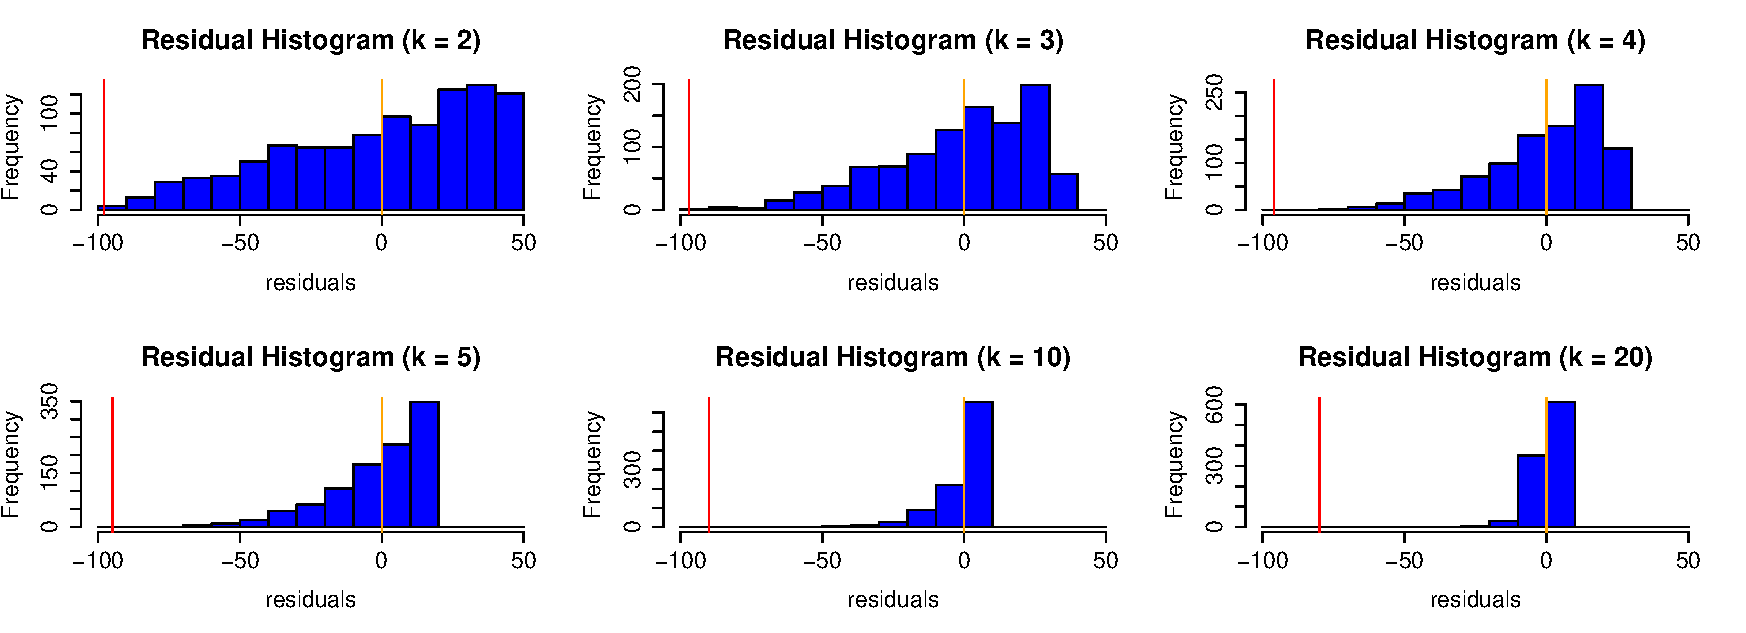
\includegraphics[width=1\textwidth, height=5cm]{residuals} 
\end{frame}

\begin{frame}
\begin{center} Thanks! \end{center} 
\pause There is much more to the problem. \\
\pause Slides and R code at \url{github.com/uberwach}
\end{frame}

\end{document}